
\chapter{Anforderungsanalyse}
\label{chapter_Anforderungsanalyse}
Das Ziel dieser Arbeit ist es, einen Teststand entwickeln, der über die Messung der Degradation von optoelektronischen Sendern. Dadurch soll eine Qualifizierung der Bauelemente erfolgen. In diesem Kapitel wird zunächst das Szenario näher beschrieben und anschließend die sich daraus entwickelnden Anforderungen definiert.

\section{Szenario}
Ein Unternehmen stellt verschiedene optoelektronischen Sensoren her. Zur Sicherstellung der Zuverlässigkeit der verwendeten \acp{LED} sollen diese mittels eines automatisierten Teststandes bezüglich ihres Degradationsverhaltens qualifiziert werden.


\begin{figure}[H]
\begin{center}
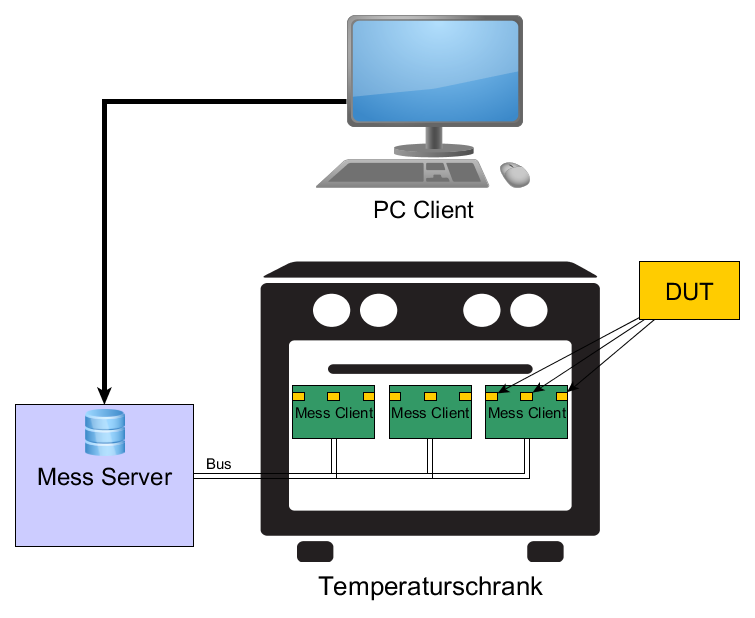
\includegraphics[scale=0.5]{img/general/Szenario.png}
\caption{Szenario}
\label{figure_Szenario}
\end{center}
\end{figure}

Der Teststand hat den in Abbildung \ref{figure_Szenario} zu sehenden Aufbau.
In einem Ofen befinden sich mehrere Mess-Clients. An diesen Mess-Clients sind jeweils 64 \acp{DUT} fest angeschlossen, bei denen das Degradationsverhalten aufgezeichnet werden soll.
Die Mess-Clients sind über einen Bus mit dem Mess-Server verbunden, welcher alle anfallenden Daten speichert.\\
Von einem PC-Client wird dann auf den Mess-Server zugegriffen um die Daten abzugreifen und grafisch auszuwerten.\\

\section{Anforderungen}

Folgende Anforderungen werden dabei an das System gestellt:
\begin{itemize}
\item Individuelle Parametrierung der \acp{DUT}
\item Automatische Erfassung der Messdaten
\item Fernzugriff auf den Mess-Server
\end{itemize}
\ \\
\textbf{Individuelle Parametrierung der \acp{DUT}}\\
Immer 64 \acp{DUT} befinden sich auf einem Mess-Client. Dabei sollen verschiedene Parameter für die \acp{DUT} berücksichtigt werden. 
Zum einen sollen die Intervalle in denen Messwerte aufgenommen werden konfigurierbar sein. Dies soll in mindestens 3 verschiedenen Intervallen möglich sein.

Beispiel: 

\begin{table}[H]
\begin{center}
\begin{tabular}{|l|l|}\hline
Zeitraum & Zeit zwischen Messungen \\ \hline
1. Woche & 12 Stunden\\ 
2. bis 4. Woche & 2 Tage\\ 

ab 5. Woche & 7 Tage\\ \hline
\end{tabular}
\caption{Intervalle}
\label{table_Intervalle}
\end{center}
\end{table}



Des Weiteren soll für jeden Mess-Client ein Pulsepattern definierbar sein. Dieses Pulsepattern wird dann als Versorgungssignal für die \acp{DUT} verwendet.

\textbf{Automatische Erfassung der Messdaten}\\
Die Messdaten der \acp{DUT} sollen zyklisch erfasst werden. Es soll die derzeitige Temperatur im Ofen, der gemessene Wert des Sensors und ein Zeitstempel gespeichert werden. Dabei sollen, wie bereits erwähnt, die Intervalle zwischen den Messungen konfigurierbar sein.\\
Für den einfachen und effizienten Zugriff auf die Daten, sollen diese in einer \ac{SQL} Datenbank abgelegt werden. Dafür ist eine Kommunikationsschnittstelle zwischen der Datenbank und den Mess-Clients erforderlich, welcher über den Mess-Server realisiert werden soll.

\textbf{Fernzugriff auf den Mess-Server}\\
Zur Auswertung der Messdaten, soll es möglich sein, von einem PC-Arbeitsplatz aus eine Verbindung zu dem Mess-Server aufzubauen. Die Messdaten sollen dann grafisch auf dem PC-Client zur Auswertung aufbereitet werden.
Auch soll ein Tunnelmodus direkten Zugriff von einem PC-Client auf einem Mess-Client ermöglichen. Dabei sollen die Parameter des Mess-Clients verändert werden können.


Diese Basis-Anforderungen und einige zusätzliche Anforderungen können wie in Tabelle \ref{table_Anforderungen} in funktionale und nicht-funktionale Anforderungen unterteilt werden.


\begin{table}[H]
\begin{center}
\begin{tabularx}{\textwidth}{|p{3cm}|X|X|X|}\hline
Art & Anforderung & Kommentar \\ \hline
Nicht-Funktional & Das System soll jederzeit verfügbar sein. & Bei Fehlern soll das System ohne große Ausfallzeit wieder Einsatzbereit sein. Zuverlässigkeit ist sehr wichtig.\\ \hline
Nicht-Funktional & Das Benutzerinterface soll zeitnah auf Anfragen reagieren. & Um Benutzerfreundlichkeit zu gewährleisten, soll auf Nutzeranfragen ohne lange Wartezeiten reagiert werden. \\ \hline
Funktional & Das System soll das Degradationsverhalten eines \ac{DUT} aufnehmen & Hauptanforderung des Systems. Messdaten sollen zu einem \ac{DUT} gesammelt werden, um den Grad der Degradation bestimmen zu können. \\ \hline
Funktional & Neue Mess-Clients sollen am PC-Client parametrierbar sein. & Parameter sollen auf dem Mess-Client und in einer Datenbank gespeichert werden. \\ \hline
Funktional & Neue bereits parametrierte Mess-Clients sollen automatisch in das System integrierbar sein. & Ein parametrierter Mess-Client kann direkt an den Bus im Ofen angeschlossen werden.\\ \hline
Funktional & Zyklische Erfassung von Messdaten. & Intervalle der Messdatenerfassung sind konfigurierbar.\\ \hline
Funktional & Messdaten sollen grafisch dargestellt werden. & Um die Daten auswerten zu können sollen sie grafisch aufbereitet werden.\\ \hline
Funktional & Die Messdaten sollen in einer Datenbank abgelegt werden. & Zum einfachen und effizienten Zugriff auf die Daten.\\ \hline
Funktional & Die Messdaten sollen via Fernzugriff erreichbar sein. & Von einem PC-Client aus, soll auf die Daten im lokalen Netzwerk zugegriffen werden können.\\ \hline
Funktional & Der Status des Systems soll ablesbar sein. & Über eine Anzeige soll das System lokal überwacht werden können.\\ \hline
Funktional & Nutzer Fehler sollen abgefangen werden. & Fehler bei der Bedienung durch den Nutzer sollen unterbunden werden.\\ \hline
\end{tabularx}
\caption{Anforderungen}
\label{table_Anforderungen}
\end{center}
\end{table}













